\chapter{Evaluation}

\section{Customer Requirements}

In this section I will evaluate whether I have fulfilled each objective which were set in my system specifications. This will determine whether the system meets the full customer requirements. Where the objectives may not have been met, I will evaluate and explain the reason for this being so. I will also provide evidence to prove that objectives have been met in other cases, which will determine that the system has acheived its specifications

%include as many subsections as necessary for your objectives
\subsection{Objective Evaluation}

%from analysis
The objectives are:
\begin{itemize}
    \item Organised layout for the database.
    \item Prevention of unnecessary duplication of data.
    \item Simple interface for entering data, meaning it can be conducted quickly.
    \item Search function to find a specific customer in the database.
    \item Ability to edit existing data easily and quickly.
    \item Ability to calculate royalties using given data
\end{itemize}

\

\subsubsection{Objective: Organised layout for the database}

This objective has been fulfilled by clearly labelling each window and giving clear table headings for each table. For example, the customer table clearly shows the following headings: "Author ID", "Firstname", "Lastname", "Email", "Phonenumber", "Address" and "Postcode". This can be seen in the image below.

\begin{figure}[H]
    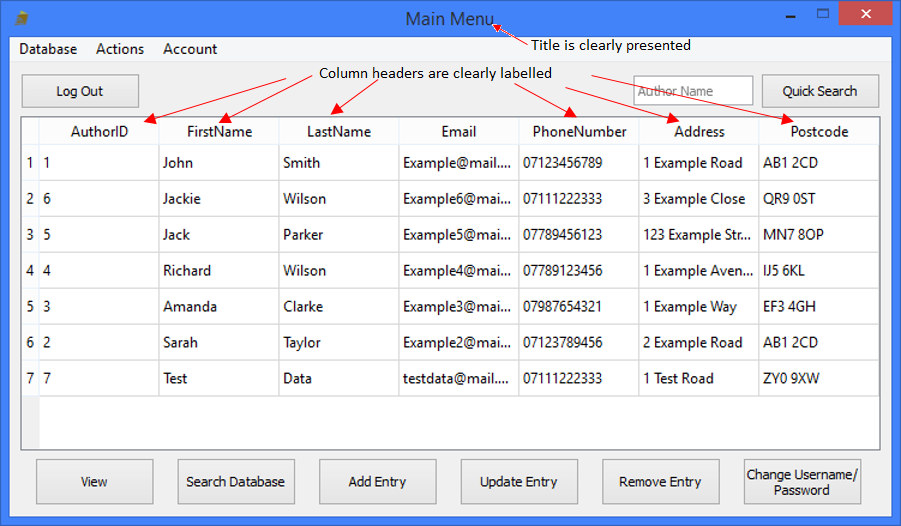
\includegraphics[width=\textwidth]{./Evaluation/Evidence/Clarity.png}
    \label{fig:InterfaceClarity} \caption{Interface is titled and tables are clearly labelled}
\end{figure}

Also, in question 1 of the questionnaire in page \pageref{fig:QuestionnairePage1}, the client has strongly agreed with the statement in the question and said that the titles on windows make the interface clear to them. The user has said that the large buttons make navigation easy as it is difficult to misclick a button. Furthermore, the headings can be clicked to sort the details by alphabetical order, ascending or descending. The tables each hold data from only 1 entity, so that the user does not get confused with the data in the table.

\

\subsubsection{Objective: Preventing Duplication}

This objective has not been fulfilled, as the system does not run checks to see whether the data is already existent in the database. The answer to question 12 of the questionnaire, on page \pageref{fig:QuestionnairePage2} shows that the user disagrees with whether the system prevents unneccessary duplication efficiently. The client has said that the system does not warn the user of the duplication, which proves that the system does not run any of these checks. However, the use of ID's still make each author unique, and the client has said the searches can be easily conducted to check whether the data is existent or not. 

\

\subsubsection{Objective: Simple interface for entering data, meaning it can be conducted quickly.}

This objective has been fulfilled, as entry boxes are clearly labelled, and there are only as many boxes as required for each entry. The entry boxes are all in line with each other, making it look tidy instead of looking cluttered. This can be seen in the image below.

\begin{figure}[H]
    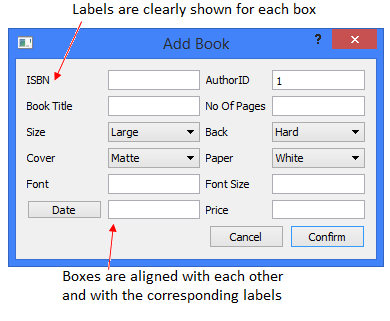
\includegraphics[width=\textwidth]{./Evaluation/Evidence/AddingInterface.png}
    \label{fig:AddingInterface} \caption{Simple interface for entering data}
\end{figure}

The client has also strongly agreed with questions 2 and 3, which show that they think that there isn't a problem with the interfaces for adding data. Each different interface for adding an certain entry has a specific title to show what is being added, which makes the current entry clear to the user.

\

\subsubsection{Objective: Search Function to find a specific customer in the database}

This objective has been fulfilled, as there are search functions in the system which can search for customers. In the images below, it is evident that the system has working search functions.

\begin{figure}[H]
    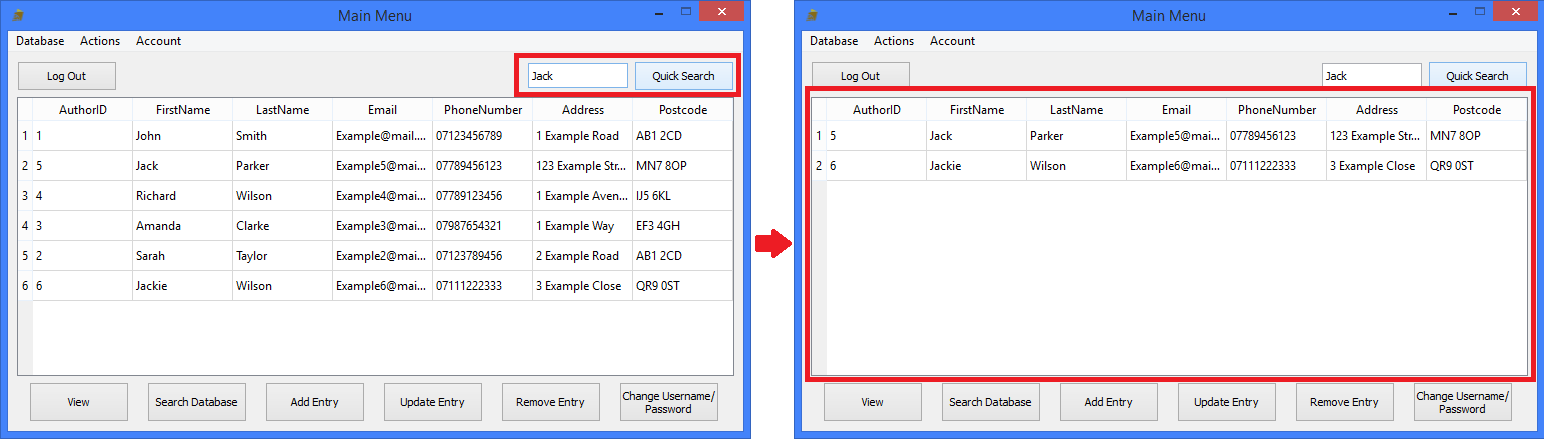
\includegraphics[width=\textwidth]{./Evaluation/Evidence/QuickSearch.png}
    \label{fig:QuickSearchFunction} \caption{Search Function which can find specific customers}
\end{figure}

\begin{figure}[H]
    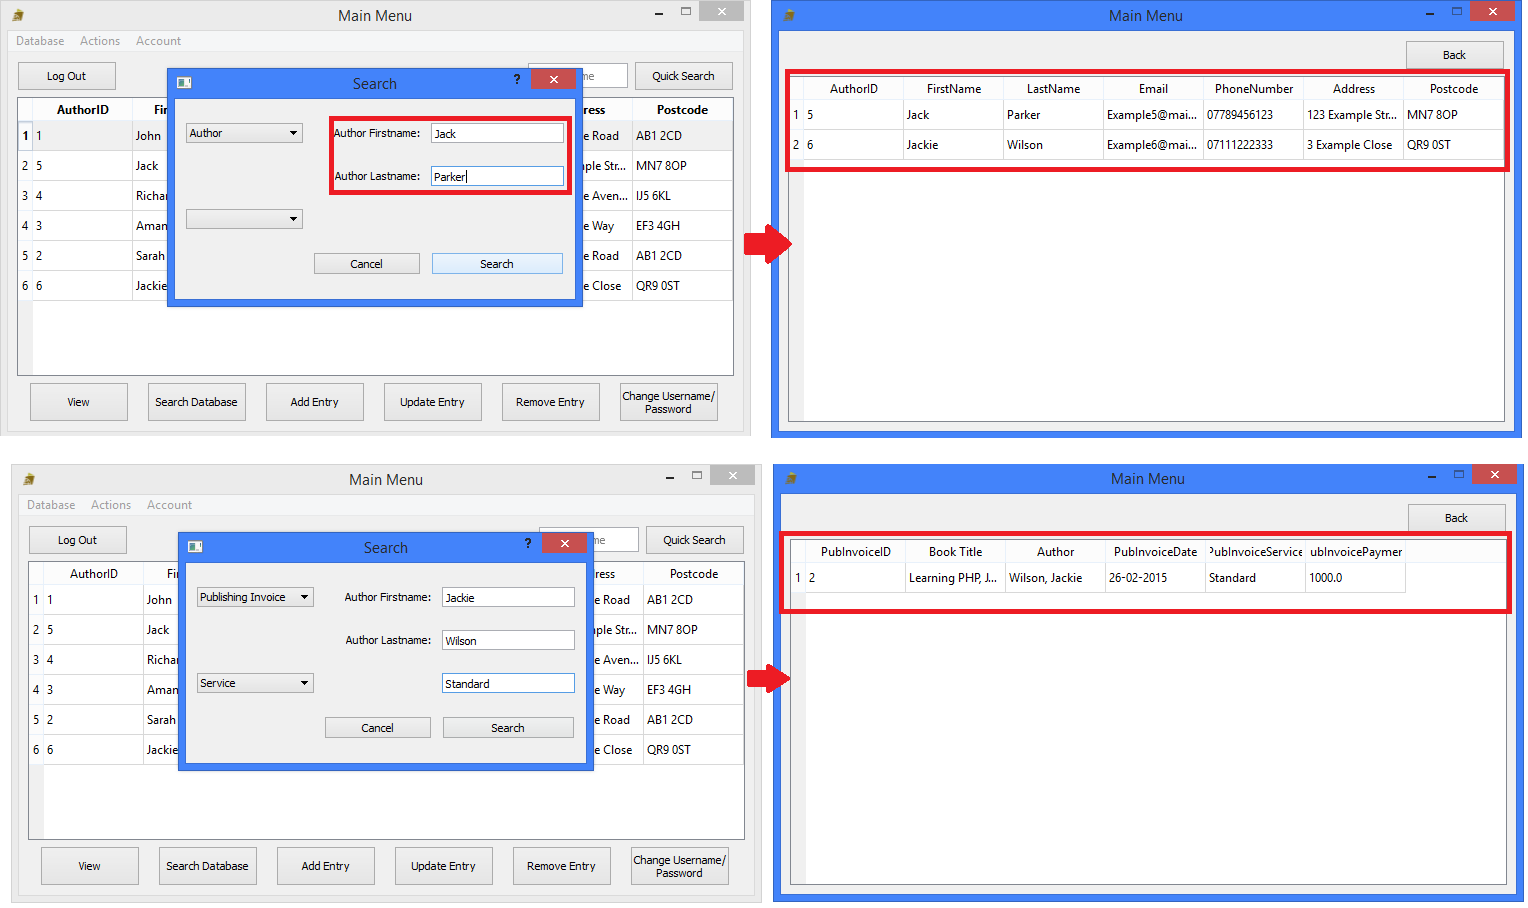
\includegraphics[width=\textwidth]{./Evaluation/Evidence/Search.png}
    \label{fig:SearchDBFunction} \caption{Search Function which can find specific customers and more}
\end{figure}

Furthermore, the client has agreed to the statement in question 4 of the questionnaire on page \pageref{fig:QuestionnairePage1}, meaning that they found the search functions up to the required standard and useful. This proves that the objective has been met. However, the data cannot be interacted with upon finding it, and this was part of the full objective of the search functionality, therefore i can conclude that this objective was partially met, even though the client was content with it.

\

\subsubsection{Objective: Ability to edit existing data easily and quickly}

This objective has been met, as all the user needs to do in the system is navigate to the data, click on it, click edit, make their changes and confirm them. This can be seen in the image below, where it is evident that the system is capable of editing data efficiently.

\begin{figure}[H]
    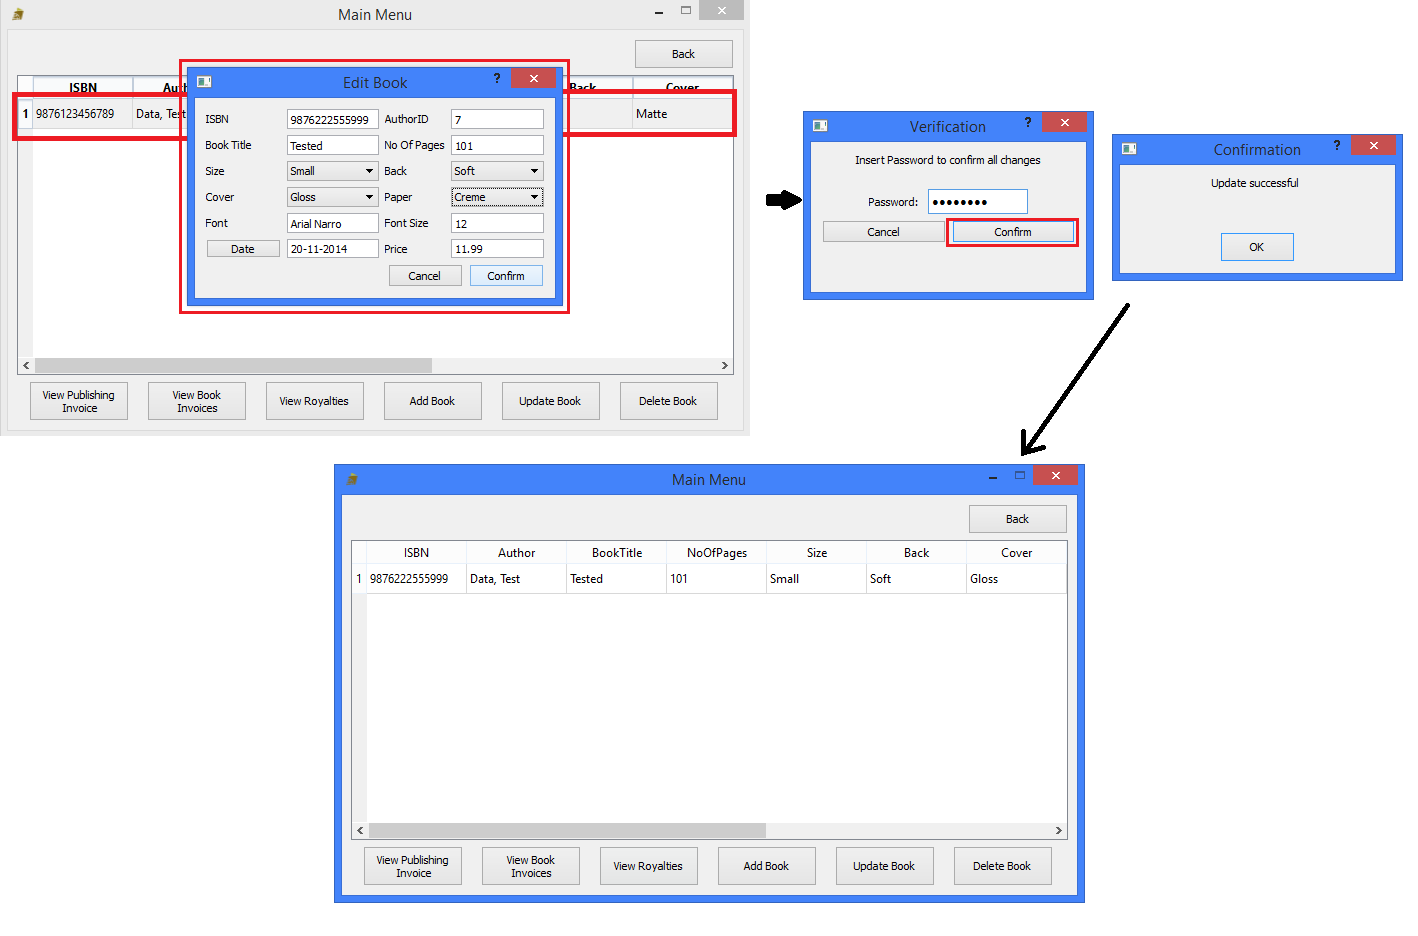
\includegraphics[width=\textwidth]{./Evaluation/Evidence/EditData.png}
    \label{fig:EditData} \caption{User finds data, clicks on it, clicks edit, makes changes, and confirms changes.}
\end{figure}

The client also strongly agreed with the statement in question 5, showing that they are content with the editing functionality in the system, and that it successfully edits and saves changes when the user verifies the changes with their credentials. This proves that the objective has been fulfilled.

\

\subsubsection{Objective: Ability to calculate royalties using given data}

This objective has been met, as the system calculates the price of a given set of items, then it sums up the prices of all the items into one royalty payment. This can be seen in the image below, where the calculations for a single set of items are displayed, and the full payment is also displayed on the royalties screen.

\begin{figure}[H]
    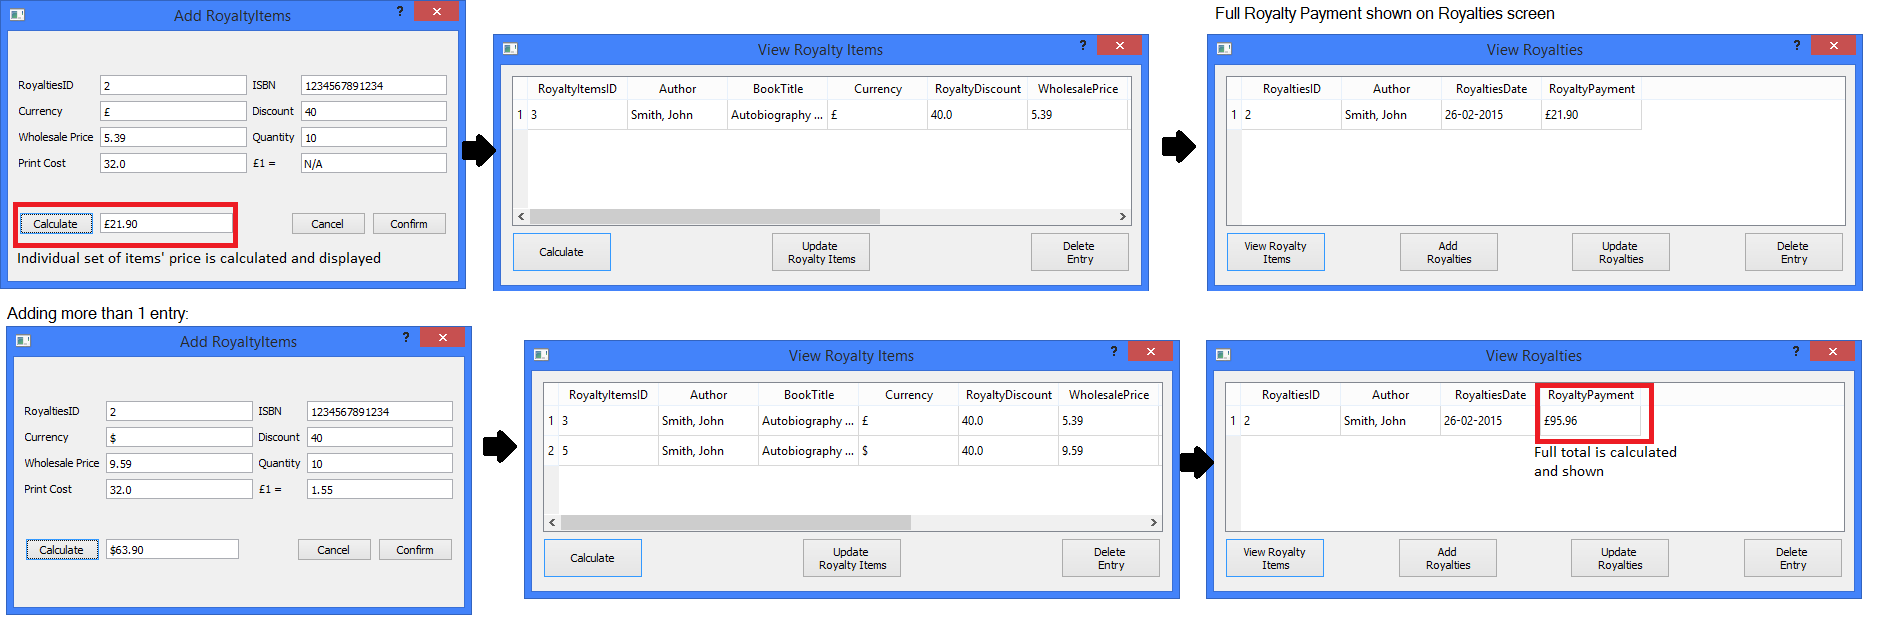
\includegraphics[width=\textwidth]{./Evaluation/Evidence/CalculateRoyalties.png}
    \label{fig:CalculateRoyalties} \caption{Individual calculations and full calculations are shown.}
\end{figure}

However, the client was merely satisfied with this functionality and this can be seen in question 14 of the questionnaire on page \pageref{fig:QuestionnairePage2}, where the client has said that they were satisfied with the fact that it completes the task set, but it is somewhat confusing as the user is required to keep track of which book they are currently interacting with. This could possibly be improved so that the customer is shown what book they are currently adding to, and can change between books somewhere on the interface, in order to avoid confusion over this. Therefore I can conclude that this objective has been mostly fulfilled.

\subsection{Summary}

The system has fulfilled half of the objectives required which were set in the system specification, and has failed to meet one of them, as seen in the graph below.

\begin{figure}[H]
    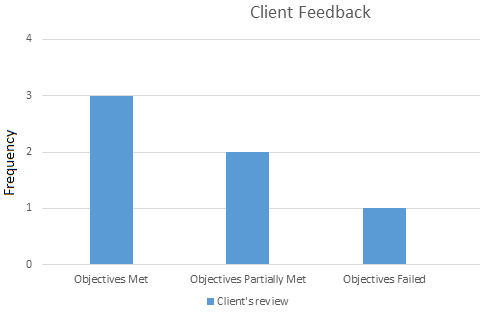
\includegraphics[width=\textwidth]{./Evaluation/ClientFeedback.png}
    \label{fig:ClientFeedback}
\end{figure}

The main reason why half of these objectives were not completely fulfilled is that I did not have enough time to finish the development of my system, which caused the validation check for duplicates in the system and the interactions with search results to be left out. However, the reason why the objective for calculations of royalty payments was not fully fulfilled is that the client was not in agreement with whether the royaly/book invoice items organisation was clear or not. This was because of how the user had to remember what book they had selected instead of it being there in front of them. The system needed to be clear on this, which it seemingly was not.

To summarise, I have concluded that the system only just meets the requirements specified by my client, because it only failed to meet 1 objective out of 6, and the objectives that were partially met were more inclined to being fully completed. Also, the client has accepted the system as they have determined that it is a major improvement on the current system that they use.

\section{Effectiveness}

%include as many subsections as necessary for your objectives
\subsection{Objective Evaluation}

\subsubsection{Objective: Organised layout for the database}

\underline{Evaluation Criteria:}

\begin{itemize}
    \item Be able to sort data in tables by date, size or alphabetical order (ascending and descending)
    \item Clear tables and fields for each entity and attribute
\end{itemize}


\underline{Verdict}

The system's organisation and clarity of layout is quite effective, as each table can be sorted by the details in the criteria above, and windows are clearly and relevantly titled. Also, headers for tables are presented in a clear manner to the user, as the table shows the headings along the top as seen in the image below.

\begin{figure}[H]
    \includegraphics[width=\textwidth]{./Evaluation/Effectiveness/OrganisedLayout.png}
    \label{fig:OrganisedLayout}
\end{figure}

Moreover, the client has said that the navigation through interfaces has been made clear with large buttons, which are relevantly labellled. This shows that the organisation of the system interfaces is effective, as it has made navigation through the system easier, which is what the objective was meant for.


\subsubsection{Objective: Simple interface for entering data}

\underline{Evaluation Criteria:}

\begin{itemize}
    \item As little amount of boxes as possible
    \item Clearly label entry boxes
\end{itemize}

\underline{Verdict}

The system's interfaces for adding data to an entity is very effective, as the interfaces only have boxes where needed, and each entry box is clearly labelled with the type of data which is required to be entered in it. This has made the user able to identify the boxes easily so that they are able to enter data without making many mistakes. This can be seen in the image below.

\begin{figure}[H]
    \includegraphics[width=\textwidth]{./Evaluation/Effectiveness/SimpleInterface.png}
    \label{fig:SimpleInterface}
\end{figure}

Furthermore, the client strongly agreed with whether the system had an effective method of adding customer data to the database. This proves that they had no problem with adding data at all, meaning that the simplicity of the interfaces have made adding data as easy it possibly could.


\subsubsection{Objective: Search function to find a specific customer in the database}

\underline{Evaluation Criteria}

\begin{itemize}
    \item Data can be found using the Author Name, or Book Title
    \item Can be edited upon finding the desired data
\end{itemize}

\underline{Verdict}

The system has partially met this objective, as the user is able to search for customers, books and book details using the search feature in the system. This has met half of the objective criteria with the addition of being able to search for data in all entities, as opposed to just a specific customer. Below is an image of an example of using the search feature to find data.

%    \item Search function to find a specific customer in the database.
%    \item Ability to edit existing data easily and quickly.
%    \item Ability to calculate royalties using given data
%\end{itemize}



\section{Learnability}

\section{Usability}

\section{Maintainability}

\section{Suggestions for Improvement}

\section{End User Evidence}

\subsection{Questionnaires} 

\begin{figure}[H]
    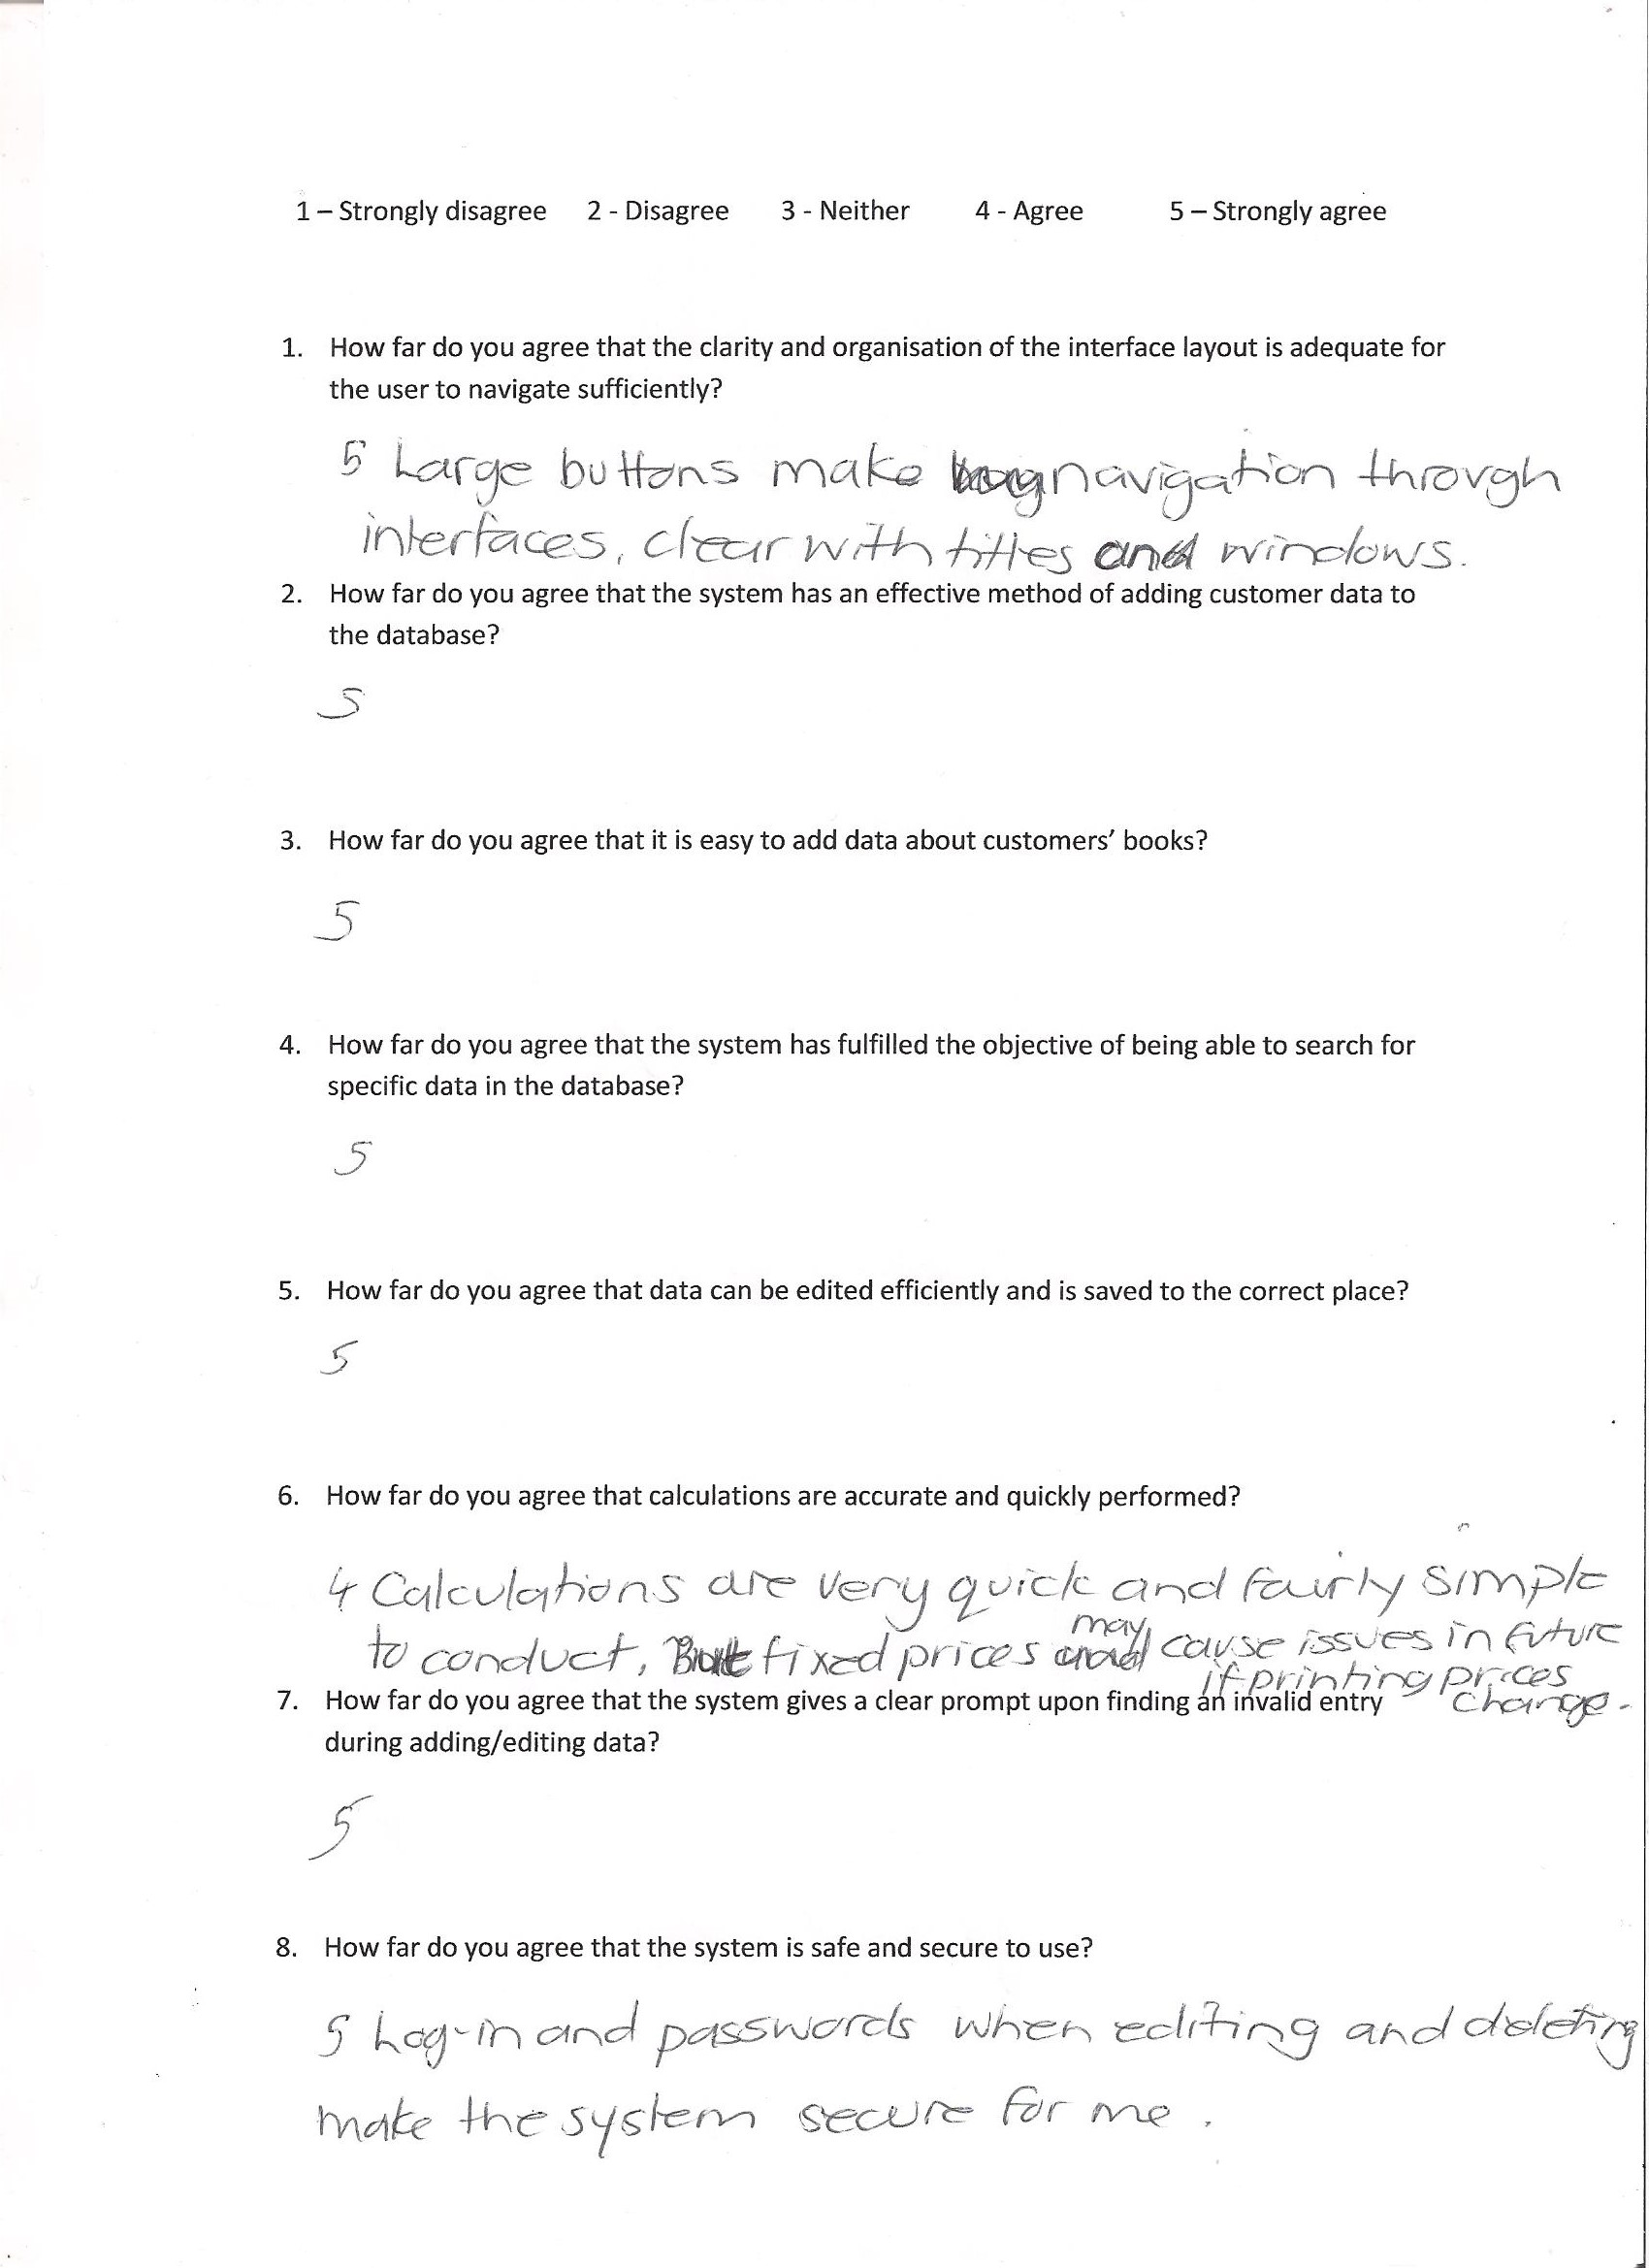
\includegraphics[width=\textwidth]{./Evaluation/Questionnaire1.png}
    \label{fig:QuestionnairePage1} \caption{Page 1 of Questionnaire}
\end{figure}

\begin{figure}[H]
    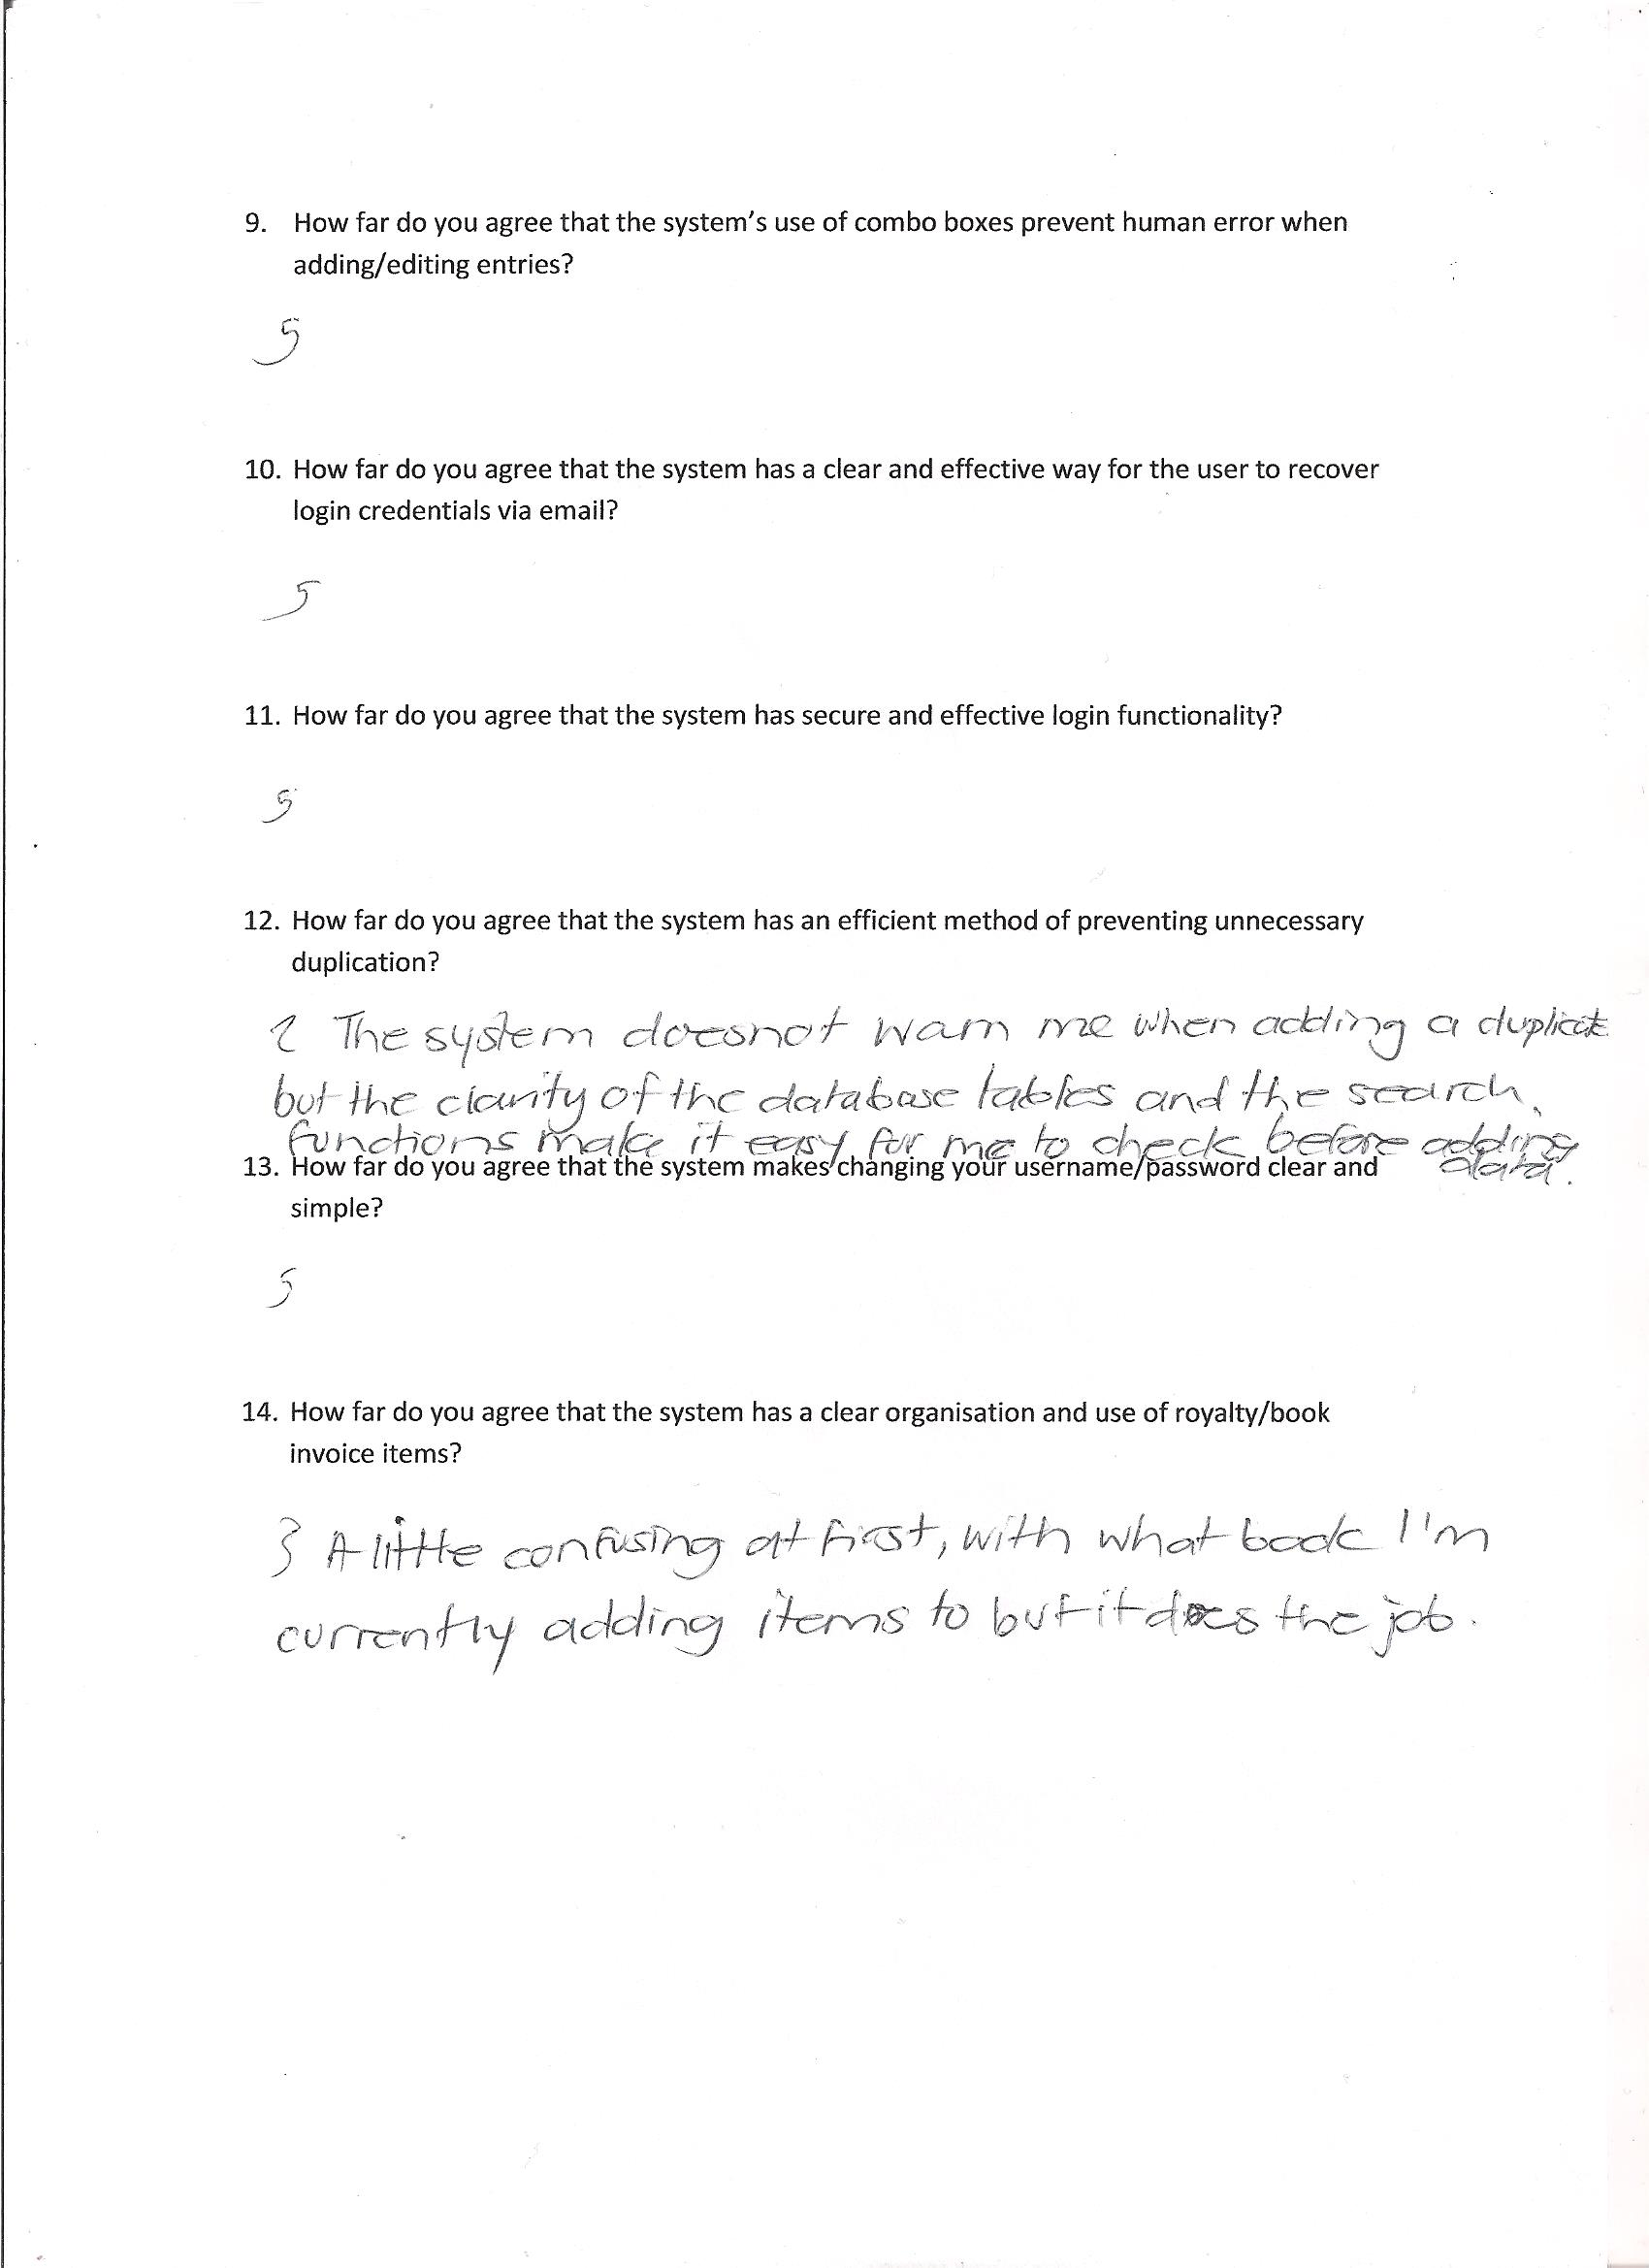
\includegraphics[width=\textwidth]{./Evaluation/Questionnaire2.png}
    \label{fig:QuestionnairePage2} \caption{Page 2 of Questionnaire}
\end{figure}

\subsection{Graphs}

\subsection{Written Statements}
